\chapter{INTRODUCTION} \label{ch:intro}

\section{Motivation}
  Given the consistent global increase in population, efficient and innovative resource utilization is increasingly important.
Our generation faces major challenges regarding food, energy, and water and must confront major issues associated with global climate change.
Growing concern for the negative environmental impacts of petroleum-based fuel has generated a market for biofuel, especially corn-based ethanol;
however, corn-based ethanol has been heavily criticized for diverting land usage away from food production, for increasing use of fertilizers and pesticides that impair water quality, and for the high carbon footprint involved in its development \cite{jones_corn-based_2015}.
Meanwhile, a great deal of unutilized coastline is available for both food and fuel production through seaweed cultivation.
Specifically, the sugar kelp \textit{Saccharina latissima} has been demonstrated to be a viable source of food, both for direct human consumption and biofuel production, especially in conjunction with other aquatic species in \textit{integrated multi-trophic aquaculture} (IMTA) \cite{brzeski_integrated_1996,chopin_integrating_2001,hadley_modeling_2015,handa_seasonal_2013}.

Furthermore, seaweed cultivation has been proposed as a nutrient remediation technique for natural waters \cite{kim_field_2014}.
Nitrogen leakage into water bodies is a significant ecological problem, and is especially relevant in close proximity to large conventional agriculture facilities and wastewater treatment plants.
Waste water treatment plants (WWTPs) in particular are facing increasingly stringent regulation of nutrients in their effluent discharges from the US Environmental Protection Agency (USEPA) and state regulatory agencies.
Nutrient management at WWTPs requires significant infrastructure, operations, and maintenance investments for tertiary treatment processes. Many treatment works are constrained financially or by space limitations in their ability to expand their operations.
As an alternative to conventional nutrient remediation techniques, the cultivation of the \textit{Saccharina latissima} within the nutrient plume of WWTP ocean outfalls has been proposed \cite{yang_kelp_2015}.
The purpose of such an undertaking would be twofold: to prevent eutrophication of the surrounding ecosystem by sequestering nutrients, and to provide supplemental nutrients that benefit macroalgae cultivation.

\begin{figure}[h]
  \centering
  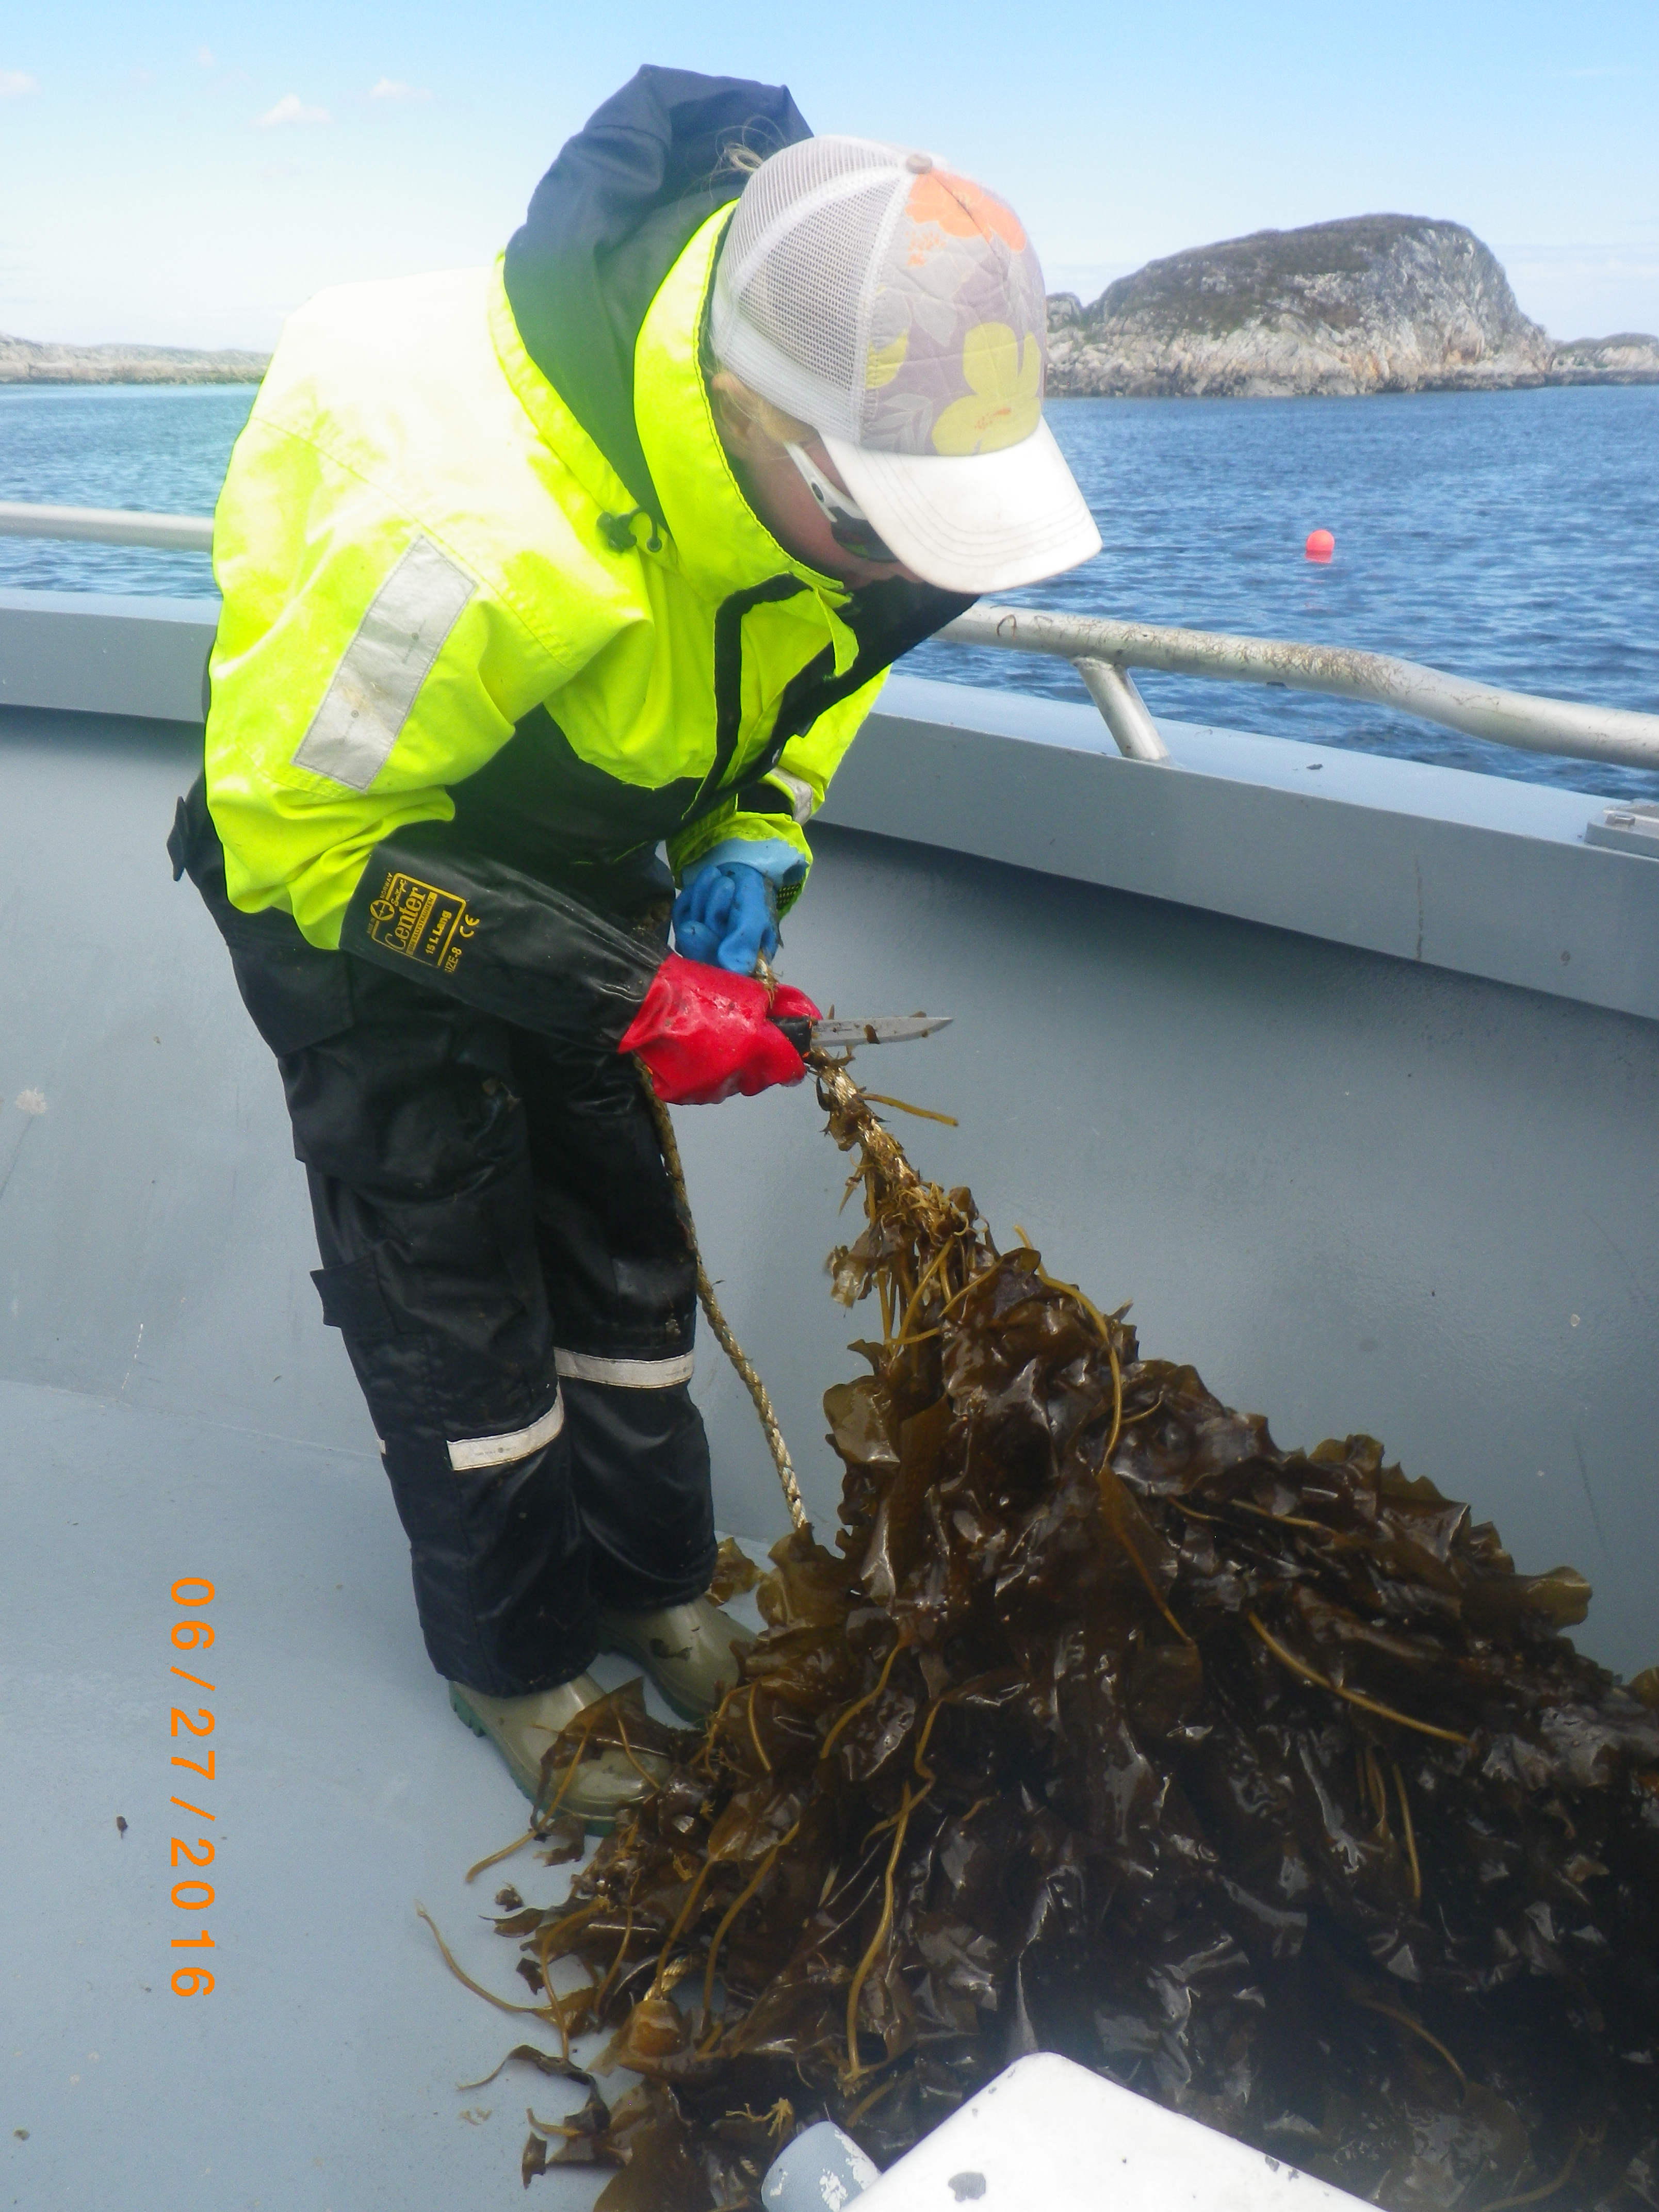
\includegraphics[width=0.5\textwidth]{kelp_photo/sonja}
  \caption{\textit{Saccharina latissima} being harvested}
  \label{fig:sonja}
\end{figure}

Large scale macroalgae cultivation has long existed in Eastern Asia due to the popularity of seaweed in Asian cuisine, and low labor costs that facilitate its manual seeding and harvest.
  More recently, less labor-intense and more industrialized kelp aquaculture has been developing in Scandinavia and in the Northeastern United States and Canada.
  For example, the MACROSEA project is a four year international research collaboration led by SINTEF, an independent research organization in Norway, and funded by the Research Council of Norway.
  The project's aim is to achieve ``successful and predictable production of high quality biomass thereby making significant steps towards industrial macroalgae cultivation in Norway''.
Figure \ref{fig:sonja} shows seaweed being harvested onboard a SINTEF research vessel.
The project includes both cultivators and scientists, working to develop a precise understanding of the full life cycle of kelp and its interaction with its environment.

A fundamental aspect of this endeavor is the development of mathematical models to describe the growth of kelp.
The development of mathematical models enables insight into a system which would be otherwise difficult or impossible to obtain.
For example, imagine that a company is interested in a new IMTA site, and is looking for a suitable location.
Running simulations to predict the potential productivity of each area would be of great assistance in choosing the best site.
Similarly, if a new cultivation technique is under consideration, simulation can estimate its viability without
having to deploy it on a large scale and risk failure or avoidable inefficiency.

Recently, a growth model \cite{broch_modelling_2012} for \textit{S. latissima} has been produced and integrated into the SINMOD \cite{wassmann_modelling_2006} hydrodynamic and ecosystem model of SINTEF.
This kelp model considers factors such as temperature, nutrient concentration, light availability, and water current.
The amount of light available is informed by spatially varying attenuation coefficients from SINMOD,
which considers optical properties of the water as well as concentrations of various organic and inorganic constituents.
However, it does not consider the effect of the kelp itself on the light field.
This is an important consideration, as high kelp densities should lead to low light levels which would inhibit further growth.
However, without accounting for self-shading, the kelp is not adequately penalized for growing too densely,
which is expected to cause overpredictions in the total biomass production.
The purpose of this thesis is to develop a first principles light model which adequately predicts the effects of self-shading on seaweed.


\section{Background on Kelp Models}

Mathematical modeling of macroalgae growth is not a new topic, although it is a reemerging one.
Several authors in the second half of the twentieth century were interested in describing the growth and composition of the macroalgae \textit{Macrocystis pyrifera}, commonly known as ``giant kelp,'' which grows prolifically off the coast of southern California.
The first such mathematical model was developed by W.J. North for the Kelp Habitat Improvement Project at the California Institute of Technology in 1968 using seven variables.
By 1974, Nick Anderson greatly expanded on North's work, and created the first comprehensive model of kelp growth which he programmed using FORTRAN \cite{anderson_mathematical_1974}.
In his model, he accounts for solar radiation intensity as a function of time of year and time of day, and refraction on the surface of the water.
He uses a simple model for shading, specifying a single parameter which determines the percentage of light that is allowed to pass through the kelp canopy floating on the surface of the water.
He also accounts for attenuation due to turbidity using Beer's Law.
Using this data on the availability of light, he calculates the photosynthesis rates and the growth experienced by the kelp.

Over a decade later in 1987, G.A.
Jackson expanded on Anderson's model for \textit{Macrocystis pyrifera} \cite{jackson_modelling_1987}, with an emphasis on including more environmental parameters and a more complete description of the growth and decay of the kelp.
The author takes into account respiration, frond decay, and sub-canopy light attenuation due to self-shading.
Light attenuation is represented with a simple exponential model, and self-shading appears as an added term in the decay coefficient.
The author does not consider radial or angular dependence on shading.
Jackson also expands Anderson's definition of canopy shading, treating the canopy not as a single layer, but as 0, 1, or 2 discrete layers, each composed of individual fronds.
While this is a significant improvement over Anderson's light model, it is still rather simplistic.

Both Anderson's and Jackson's model were carried out by numerically solving a system of differential equations over small time intervals.
In 1990, M.A. Burgman and V.A. Gerard developed a stochastic population model \cite{burgman_stage-structured_1990}.
This approach functions by dividing kelp plants into groups based on size and age and generating random numbers to determine how the population distribution over these groups changes over time based on measured rates of growth, death, decay, light availability, etc.
In the same year, Nyman et. al. \cite{nyman_macrocystis_1990} published a similar model alongside a Markov chain model, and compared the results with experimental data collected in New Zealand.

In 1996 and 1998 respectively, P. Duarte and J.G. Ferreira used the size-class approach to create a more general model of macroalgae growth, and Yoshimori et. al. created a differential equation model of \textit{Laminaria religiosa} with specific emphasis on temperature dependence of growth rate \cite{duarte_model_1997,yoshimori_mathematical_1998}.
These were some of the first models of kelp growth that did not specifically relate to \textit{Macrocystis pyrifera} (``giant kelp'').

The model developed by Broch et. al. at SINTEF \cite{broch_modelling_2012, broch_modelling_2013, handa_seasonal_2013} uses a super-individual approach, whereby a small number of individual kelp fronds are explicitly simulated at several discrete depth layers.
Each super-individual is assumed to represent a certain number of actual individuals in the population.
The number of individuals represented by each super-individual may change over the course of the simulation due to population loss.
The super-individual approach has the advantage of capturing some of the dynamics at the individual scale, while compromising full detail for the sake of reduced computational cost.

\section{Background on Radiative Transfer}
In terms of optical quantities, of primary interest is the radiance, which describes the rate of energy flow through each point in space in \textit{each} direction.
Irradiance, on the other hand, describes the total energy flow through a point in space over \textit{every} direction, and is calculated by integrating radiance over all angles.
Irradiance, in turn, determines the photosynthetic rate of the kelp, and therefore the total amount of biomass producible in a given area as well as the total nutrient remediation potential.
The equation governing the radiance throughout the system is known as the radiative transfer equation (RTE), which has been used extensively in stellar astrophysics \cite{chandrasekhar_radiative_1960,petkova_novel_2011}; its application to marine biology is fairly recent \cite{mobley_radiative_2001}.
In its full form, radiance is a function of 3 spatial dimensions, 2 angular dimensions, and frequency, making for a formidable problem.
In this work, frequency is ignored; only the total radiation in the photosynthetic spectrum, known as photosynthetically active radiation (PAR), is considered.
The RTE states that along a given path, radiance is decreased by absorption and scattering out of the path, while it is increased by emission and scattering into the path.
In the case of macroalgae cultivation, emission is negligible, owing only perhaps to some small luminescent phytoplankton or other anomaly, and can therefore be safely ignored.
However, the emission term will be retained in the calculations of this thesis, as it is mathematically useful to verify the correctness of the solution algorithm.

\section{Overview of Thesis}
The remainder of this document is organized as follows.
In Chapter \Rom{\ref{chap:kelp}}, a probabilistic model is developed to describe the spatial distribution of kelp by assuming simple distributions for the lengths and orientations of fronds.
Chapter \Rom{\ref{chap:light}} begins with a survey of fundamental radiometric quantities and optical properties of matter.
The spatial kelp distribution from Chapter \Rom{\ref{chap:kelp}} is used to determine optical properties of the combined water-kelp medium,
and the radiative transfer equation, an integro-partial differential equation which describes the the light field as a function of position and angle, is discussed.
An asymptotic expansion is explored for the case of low scattering, allowing for analytical, ordered approximations to the true light field.
In Chapter \Rom{\ref{chap:numerical}}, details are given for the numerical solution of the equations from Chapters \Rom{\ref{chap:kelp}} and \Rom{\ref{chap:light}}.
Both the full finite difference solution and the asymptotic approximation are thoroughly developed.

Chapter \Rom{\ref{chap:model_analysis}} is an in--depth discussion of sources of error in both solution procedures.
The concepts of verifying codes in general as well as specific calculations are discussed.
Exact discretization errors are calculated via the method of manufactured solutions in order to demonstrate
that the methods exhibit convergence properties which build confidence in their correctness.
A method for estimating errors for realistic cases is also developed.

Next, Chapter \Rom{\ref{chap:application}} surveys practical considerations to keep in mind when applying the algorithms in real situations.
Relevant model parameter values from the literature are collected, and estimates are given for those not readily available.
Following that is a set of guidelines for choosing which algorithm and which algorithm parameters to use based on the optical scenario to be simulated.
Advantages and disadvantages of both approaches are presented.
While the finite difference technique can be applied to any situation, it often requires prohibitively large CPU and memory resources, whereas the numerical asymptotic solution is generally faster and its memory footprint never exceeds the capacity of a standard laptop for reasonable grid sizes.
The Chapter concludes with a comparison to other two simpler light models, and specific qualitative differences are noted.
As expected, the presence of self-shading in this model results in the prediction of lower light levels regions of high kelp density.
However, the presence of scattering in the model increases light levels elsewhere, especially near the surface of the water.

Finally, Chapter \Rom{\ref{chap:conclusion}} concludes the thesis by briefly summarizing the model, discussing its achievements and limitations, and suggesting improvements and avenues for future work.
Several appendices follow with further details about the algorithm, as well as the full source code of the Fortran model developed.
